\documentclass{beamer}

\usepackage[utf8x]{inputenc}
\usepackage[OT4]{fontenc}

\usetheme[bullet=circle,
          titleline=true,
          pageofpages=of,
          alternativetitlepage=true]{Torino}

\usepackage{color}

\usepackage{ragged2e}
\usepackage{hyphenat}

\usepackage{amsmath}
\usepackage{amsfonts}
\usepackage{amsthm}

%\usepackage{sympytex}
\usepackage{pythonhighlight}

\definecolor{MyGreen}{rgb}{0.40,0.80,0.20}

\title{SymPy --- a library for symbolic mathematics \linebreak in pure Python}
\author{Mateusz Paprocki \texttt{<mattpap@gmail.com>}}
\institute[PWR]{Wrocław University of Technology \linebreak SymPy Development Team}
\date{\today}

\newenvironment{jblock}[1]{
    \begin{block}{#1}\justifying\nohyphens
}{
    \end{block}
}

\begin{document}

\setbeamercovered{transparent}

\frame{\titlepage}

\begin{frame}[fragile]
    \frametitle{What is SymPy?}

    \begin{itemize}
        \item A pure Python library for symbolic mathematics
        %\item A \structure<2>{pure} \structure<3>{Python} \structure<4>{library}
        %      for \structure<5>{symbolic} \structure<6>{mathematics}
    \end{itemize}

    \onslide<2->
    \begin{python}
  >>> from sympy import *
  >>> x = Symbol('x')

  >>> limit(sin(pi*x)/x, x, 0)
  pi

  >>> integrate(x + sinh(x), x)
  (1/2)*x**2 + cosh(x)

  >>> diff(_, x)
  x + sinh(x)
    \end{python}
\end{frame}

\begin{frame}[fragile]
    \frametitle{Why reinvent the wheel for the 37th time?}

    \onslide<1->{
        There are numerous symbolic manipulation systems:
        \begin{itemize}
            \item \structure{Proprietary} software:
                \begin{itemize}
                    \item Mathematica, Maple, Magma, \ldots
                \end{itemize}
            \item \structure{Open Source} software:
                \begin{itemize}
                    \item AXIOM, GiNaC, Maxima, PARI, Sage, Singular, Yacas, \ldots
                \end{itemize}
        \end{itemize}
    }

    \onslide<2->{
        {\color{red} Problems:}
        \begin{itemize}
            \item all \structure{invent} their own \structure{language}
                \begin{itemize}
                    \item need to learn yet another language
                    \item separation into core and library
                    \item hard to extend core functionality
                    \item \structure{except}: GiNaC and Sage
                \end{itemize}
            \item all need quite some time to compile
                \begin{itemize}
                    \item slow development cycle
                \end{itemize}
        \end{itemize}
    }
\end{frame}

\begin{frame}[fragile]
    \frametitle{What we want to achieve?}

    \begin{itemize}
        \item<1-> pure Python library
            \begin{itemize}
                \item no new environment, language, \ldots
                \item works out of the box on any platform
                \item non Python modules could be optional
            \end{itemize}
        \item<2-> simple design
            \begin{itemize}
                \item small code base
                \item easy to extend
            \end{itemize}
        \item<3-> rich functionality
            \begin{itemize}
                \item support most important fields of mathematics
                \item implement modern algorithms, e.g. Gruntz algorithm
            \end{itemize}
        \item<4-> use Cython for time critical code
            \begin{itemize}
                \item optional, accompanying the interpreted version
            \end{itemize}
        \item<5-> liberal licence: BSD
            \begin{itemize}
                \item freedom on ways of using SymPy
            \end{itemize}
    \end{itemize}
\end{frame}

\begin{frame}[fragile]
    \frametitle{Why we chose Python?}

    \begin{itemize}
        \item<1-> widely used language
            \begin{itemize}
                \item Google, NASA, \ldots
            \end{itemize}
        \item<2-> very clean language
            \begin{itemize}
                \item simple syntactics and semantics
                \item usually one way to do things
                \item easy to read and maintain
            \end{itemize}
        \item<3-> huge number of libraries
            \begin{itemize}
                \item numerical computation: NumPy, SciPy
                \item physics, simulation, bioinformatics
                \item visualisation, 3D graphics, plotting
                \item databases, networking, \ldots
            \end{itemize}
        \item<4-> easy to bind with other code
            \begin{itemize}
                \item C/C++ via native API or Cython
                \item Fortran using f2py bindings
            \end{itemize}
    \end{itemize}
\end{frame}

\begin{frame}[fragile]
    \frametitle{But wait, there is Sage \ldots}

    \onslide<1->{
        Sage aims to:
        \begin{itemize}
            \item create a viable \structure{free open source alternative} to Maple, \\ Mathematica, Matlab and Magma
            \item \structure{glue together} useful mathematics software packages \\ and provide transparent interface to them
        \end{itemize}
    }

    \begin{itemize}
        \item<2-> {\color{red} Cons:}
            \begin{itemize}
                \item difficult to use as a library
                \item Sage is a software distribution
                \item very large in size and with long build times
                \item Sage prefers to use a preparser (it can be turned off)
            \end{itemize}
        \item<3-> {\color{MyGreen} Pros:}
            \begin{itemize}
                \item it includes most recent version of SymPy
                \item nice interface to lots of packages, easy to install
            \end{itemize}
    \end{itemize}
\end{frame}

\begin{frame}[fragile]
    \frametitle{Sage vs SymPy}

    \begin{itemize}
        \item \structure{Sage} example:
            \begin{python}
sage: limit(sin(x)/x, x=0)
1
sage: integrate(x+sinh(x), x)
cosh(x) + x^2/2
            \end{python}
        \vskip+0.5cm
        \item \structure{SymPy} example:
            \begin{python}
In [1]: limit(sin(x)/x, x, 0)
Out[1]: 1
In [2]: integrate(x+sinh(x), x)
Out[2]: (1/2)*x**2 + cosh(x)
            \end{python}
    \end{itemize}
\end{frame}

\begin{frame}[fragile]
    \frametitle{Capabilities}
    \framesubtitle{What SymPy can do?}

    \begin{columns}
        \begin{column}[l]{0.5\textwidth}
            \begin{itemize}
                \item core functionality
                    \begin{itemize}
                        \item differentiation, truncated series
                        \item pattern matching, substitutions
                        \item non--commutative algebras
                        \item assumptions engine, logic
                    \end{itemize}
                \item symbolic \ldots
                    \begin{itemize}
                        \item integration, summation
                        \item limits
                    \end{itemize}
                \item polynomial algebra
                    \begin{itemize}
                        \item Gröbner bases computation
                        \item multivariate factorization
                    \end{itemize}
                \item matrix algebra
            \end{itemize}
        \end{column}
        \begin{column}[r]{0.5\textwidth}
            \begin{itemize}
                \item equations solvers
                    \begin{itemize}
                        \item algebraic, transcendental
                        \item recurrence, differential
                    \end{itemize}
                \item systems solvers
                    \begin{itemize}
                        \item linear, polynomial
                    \end{itemize}
                \item pretty--printing
                    \begin{itemize}
                        \item Unicode, ASCII
                        \item LaTeX, MathML
                    \end{itemize}
                \item 2D \& 3D plotting
                \item \structure{\ldots}
            \end{itemize}
        \end{column}
    \end{columns}
\end{frame}

\begin{frame}[fragile]
    \frametitle{ASCII pretty--printing}

    \begin{center}
        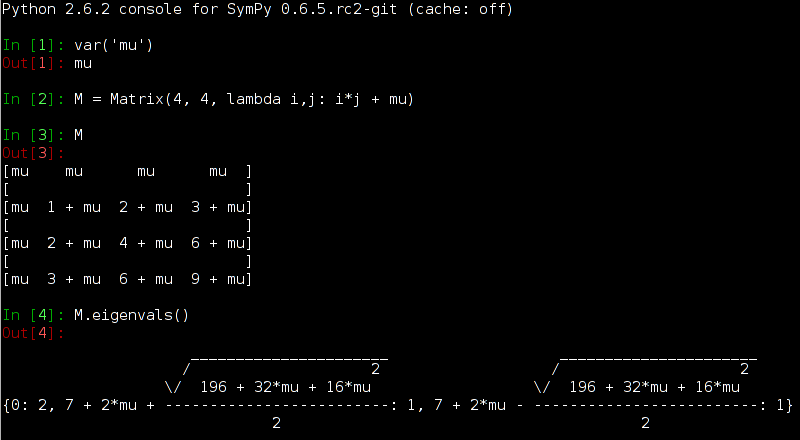
\includegraphics[scale=0.65]{images/sympy-ascii.png}
    \end{center}
\end{frame}

\begin{frame}[fragile]
    \frametitle{Unicode pretty--printing}

    \begin{center}
        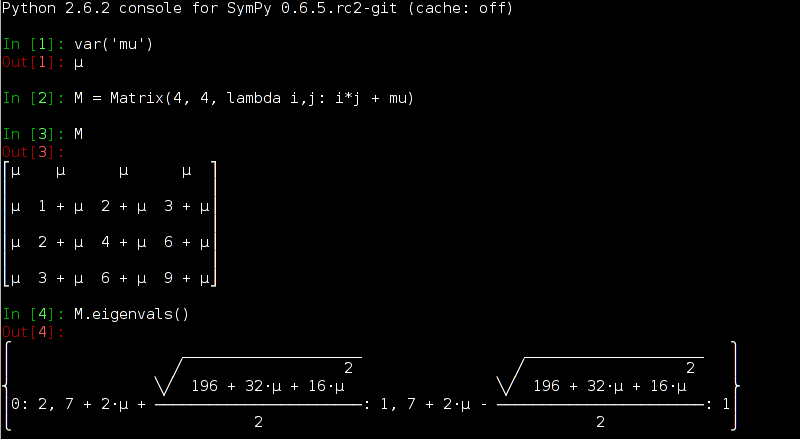
\includegraphics[scale=0.65]{images/sympy-unicode.png}
    \end{center}
\end{frame}


\begin{frame}[fragile]
    \frametitle{List of SymPy's modules (1)}

    \begin{description}
        \item[concrete] symbolic products and summations
        \item[core] Basic, Add, Mul, Pow, Function, \structure{\ldots}
        \item[functions] elementary and special functions
        \item[galgebra] geometric algebra
        \item[geometry] geometric entities
        \item[integrals] symbolic integrator
        \item[interactive] for setting up pretty--printing
        \item[logic] new assumptions engine, boolean functions
        \item[matrices] Matrix class, orthogonalization etc.
        \item[mpmath] fast arbitrary precision numerical math
    \end{description}
\end{frame}

\begin{frame}[fragile]
    \frametitle{List of SymPy's modules (2)}

    \begin{description}
        \item[ntheory] number theoretical functions
        \item[parsing] Mathematica and Maxima parsers
        \item[physics] physical units, Pauli matrices
        \item[plotting] 2D and 3D plots using pyglet
        \item[polys] polynomial algebra, factorization
        \item[printing] pretty-printing, code generation
        \item[series] compute limits and tructated series
        \item[simplify] rewrite expresions in other forms
        \item[solvers] algebraic, recurrence, differential
        \item[statistics] standard probability distributions
        \item[utilities] test framework, compatibility stuff
    \end{description}
\end{frame}

\begin{frame}[fragile]
    \frametitle{Internals}
    \framesubtitle{So, how does SymPy work?}

    \begin{python}
In [1]: 7
Out[1]: 7

In [2]: type(_)
Out[2]: <type 'int'>

In [3]: sympify(7)
Out[3]: 7

In [4]: type(_)
Out[4]: <class 'sympy.core.numbers.Integer'>

In [5]: sympify('factor(x**5+1, x)')
Out[5]: (1 + x)*(1 - x + x**2 - x**3 + x**4)
    \end{python}
\end{frame}

\begin{frame}[fragile]
    \frametitle{Internals}
    \framesubtitle{Object oriented model}

    \begin{columns}
        \begin{column}[r]{0.3\textwidth}
            \begin{itemize}
                \item Basic
                \begin{itemize}
                    \item Add
                    \item Mul
                    \item Pow
                    \item Symbol
                    \item Integer
                    \item Rational
                    \item Function
                        \begin{itemize}
                            \item sin
                            \item cos
                            \item \structure{\ldots}
                        \end{itemize}
                \end{itemize}
            \end{itemize}
        \end{column}
        \begin{column}[r]{0.6\textwidth}
            Each class has \verb+__new__+ method:
            \begin{itemize}
                \item automatic simplification of arguments
                \item no intermediate classes construction
            \end{itemize}
            \vskip+0.5cm
            Example:
            \begin{itemize}
                \item \pyth!Add(Add(x, y), x)! becomes \pyth!Add(Mul(2, x), y)!
            \end{itemize}
        \end{column}
    \end{columns}

\end{frame}

\begin{frame}[fragile]
    \frametitle{Internals}
    \framesubtitle{Automatic expression evaluation}

    \begin{python}
In [1]: Add(x, 7, x, y, -2)
Out[1]: 5 + y + 2*x

In [2]: x + 7 + x + y - 2
Out[2]: 5 + y + 2*x

In [3]: Mul(x, 7, x, y, 2)
Out[3]: 14*y*x**2

In [4]: x*7*x*y*2
Out[4]: 14*y*x**2

In [5]: sin(2*pi)
Out[5]: 0
    \end{python}

\end{frame}

\begin{frame}[fragile]
    \frametitle{Example}
    \framesubtitle{Computing minimal polynomial of an algebraic number (1)}

    \begin{python}
In [1]: from sympy import *

In [2]: y = sqrt(2) + sqrt(3) + sqrt(6)

In [3]: var('a,b,c')
Out[3]: (a, b, c)

In [4]: f = [a**2 - 2, b**2 - 3, c**2 - 6, x - a-b-c]

In [5]: G = groebner(f, a,b,c,x, order='lex')

In [6]: G[-1]
Out[6]: 529 - 1292*x**2 + 438*x**4 - 44*x**6 + x**8

In [7]: F = factors(_, x)[1]
    \end{python}
\end{frame}

\begin{frame}[fragile]
    \frametitle{Example}
    \framesubtitle{Computing minimal polynomial of an algebraic number (2)}

    \begin{python}
In [8]: len(F)
Out[8]: 2

In [9]: (u, _), (v, _) = F

In [10]: u
Out[10]: 23 - 48*x + 22*x**2 - x**4

In [11]: simplify(u.subs(x, y))
Out[11]: -96*2**(1/2) - 96*3**(1/2) - 96*6**(1/2)

In [12]: v
Out[12]: 23 + 48*x + 22*x**2 - x**4

In [13]: simplify(v.subs(x, y))
Out[13]: 0
    \end{python}
\end{frame}

\begin{frame}[fragile]
    \frametitle{But wait, isn't this slow?}
    \framesubtitle{Lets compare SymPy with SAGE (1)}

    Sum of terms in the following form:
    \begin{equation*}
    x^k (k y)^{2 k} z^{y^k}, k \in [1,200]
    \end{equation*}

    \begin{python}
In [1]: f = lambda k: x**k*(k*y)**(2*k)*z**y**k
In [2]: %timeit a = Add(*map(f, xrange(1, 200)))
10 loops, best of 3: 146 ms per loop
    \end{python}

    \begin{python}
sage: f = lambda k: x**k*(k*y)**(2*k)*z**y**k
sage: %timeit a = sum(map(f, xrange(1, 200)))
10 loops, best of 3: 30.9 ms per loop
    \end{python}
\end{frame}

\begin{frame}[fragile]
    \frametitle{But wait, isn't this slow?}
    \framesubtitle{Lets compare SymPy with SAGE (2)}

    Sum of terms in the following form:
    \begin{equation*}
    sin(k x)^k (k \cdot cos(k y))^{2 k}, k \in [1,200]
    \end{equation*}

    \begin{python}
In [3]: g = lambda k: sin(k*x)**k*(k*cos(k*y))**(2*k)
In [4]: %timeit a = Add(*map(g, xrange(1, 200)))
10 loops, best of 3: 527 ms per loop
    \end{python}

    \begin{python}
sage: g = lambda k: sin(k*x)**k*(k*cos(k*y))**(2*k)
sage: %timeit a = sum(map(g, xrange(1, 200)))
10 loops, best of 3: 38.6 ms per loop
    \end{python}
\end{frame}

\begin{frame}[fragile]
    \frametitle{But wait, isn't this slow?}
    \framesubtitle{Lets compare SymPy with SAGE (3)}

    \onslide<1->
    Cyclotomic factorization of a polynomial:
    \begin{python}
In [5]: %timeit a = factor(x**462 + 1)
10 loops, best of 3: 215 ms per loop
    \end{python}
    \begin{python}
sage: %timeit a = factor(x**462 + 1)
10 loops, best of 3: 637 ms per loop
    \end{python}

    \onslide<2->
    Factorization of a multivariate polynomial:
    \begin{python}
In [6]: %timeit a = factor(x**20 - z**5*y**20)
10 loops, best of 3: 614 ms per loop
    \end{python}
    \begin{python}
sage: %timeit a = factor(x**20 - z**5*y**20)
10 loops, best of 3: 44.4 ms per loop
    \end{python}
\end{frame}

\begin{frame}[fragile]
    \frametitle{What can be done to improve speed?}

    \begin{itemize}
        \item use better algorithms, if available, e.g.
        \begin{itemize}
            \item use modular techniques in polynomial problems
        \end{itemize}
        \item rewrite core modules in \structure{Cython}
        \begin{itemize}
            \item better (?): use \structure{pure mode}
\begin{python}
import cython

@cython.locals(i=cython.int)
cpdef divisors(int n)
\end{python}
        \end{itemize}
        \item improve CPython, e.g.
        \begin{itemize}
            \item see \structure{unladen--swallow} project
        \end{itemize}
    \end{itemize}
\end{frame}

\begin{frame}[fragile]
    \frametitle{Our workflow}

    \begin{itemize}
        \item we use GIT for source code management
            \begin{itemize}
                \item there is one official repository with master branch
                \item each developer has a development repository
                \item patch review + branch tracking
            \end{itemize}
        \item each public function must have
        \begin{itemize}
            \item a test suite associated
            \item a docstring written
            \item examples prepared
        \end{itemize}
        \item all tests must pass in the official repository
        \item we use buildbots to test different architectures
        \begin{itemize}
            \item amd64-py2.4, amd64-py2.5, amd64-py2.6
            \item i386-py2.4, i386-py2.5, i386-py2.6
            \item amd64-py2.5-Qnew-sympy-tests
        \end{itemize}
        \item we use ReST to write documentation
    \end{itemize}
\end{frame}

\begin{frame}[fragile]
    \frametitle{Contact}
    \framesubtitle{How to get involved?}

    \begin{itemize}
        \item Visit our main web site:
            \begin{itemize}
                \item \texttt{www.sympy.org}
            \end{itemize}
        \item and additional web sites:
            \begin{itemize}
                \item \texttt{wiki.sympy.org}
                \item \texttt{docs.sympy.org}
                \item \texttt{live.sympy.org}
            \end{itemize}
        \item Contact us on our mailing list:
            \begin{itemize}
                \item \texttt{sympy@googlegroups.com}
            \end{itemize}
        \item or/and IRC channel:
            \begin{itemize}
                \item \texttt{\#sympy} on FreeNode
            \end{itemize}
        \item Clone source repository:
        \begin{verbatim}
        git clone git://git.sympy.org/sympy.git
        \end{verbatim}
    \end{itemize}
\end{frame}

\begin{frame}
    \frametitle{Conclusion}

    \begin{itemize}
        \item<1-> What \structure{is} done:
            \begin{itemize}
                \item basic core functionality and class structure
                \item algorithms for most fields of mathematics
                \item efficient workflow established
                \begin{itemize}
                    \item GIT + patch review
                \end{itemize}
            \end{itemize}
        \item<2-> What \structure{is not} done:
            \begin{itemize}
                \item full test coverage
                \item optimizations
                \item robust
                \begin{itemize}
                    \item integrator
                    \item assumptions engine
                    \item ODE and PDE solvers, \structure{\ldots}
                \end{itemize}
            \end{itemize}
        \item<3-> What \structure{won't be} done:
            \begin{itemize}
                \item GUI, notebook etc.
            \end{itemize}
    \end{itemize}
\end{frame}

\begin{frame}
    \begin{center}
        \textbf{\LARGE Thank you for your attention!}
        \linebreak
        \vskip+0.5cm
        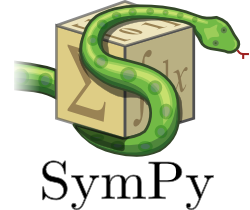
\includegraphics[scale=0.2]{images/sympy-250px.png}
    \end{center}
\end{frame}

%\begin{frame}%[allowframebreaks]
%    \frametitle{References}
%
%    \nocite{*}
%    \bibliographystyle{acm}
%    \bibliography{euroscipy-slides-2009}
%\end{frame}

\end{document}

